% this file is called up by thesis.tex
% content in this file will be fed into the main document

%: ----------------------- name of chapter  -------------------------
\chapter{Appendix A: Some Results in Algebraic Geometry}\label{serre_duality} % top level followed by section, subsection


%: ----------------------- paths to graphics ------------------------

% change according to folder and file names
\ifpdf
    \graphicspath{{figures/}{figures/}{figures/}}
\else
    \graphicspath{{figures/}{figures/}}
\fi

%: ----------------------- contents from here ------------------------

In this Appendix we collect a number of technical results which are exploited in various parts of the Thesis, a solution adopted with the objective of making the main text lighter and more readable.\\ 
For some of the statements a direct proof is given in these pages, while for others we refer to the literature, giving precise references.

\section{Degeneracy loci}
	
	Recall from Section \ref{sec:fitt_deg} the definition of degeneracy ideals $I_n \ph$. A result by Eagon and Northcott on the height of such ideals is exploited in Section \ref{sec:lower_bound} to obtain a lower bound for the dimension of connected components of the varieties \modu.
	\begin{theo}\label{thm:height}
		Let $\ph:E\to F$ be a morphism of locally free sheaves of finite rank $e$ and $f$. Then for every $\mathfrak{p}$ a minimal prime ideal of $I_n \ph$ we have
		$$ \height (\mathfrak{p}) \leq (e-n+1)(f-n+1). $$
	\end{theo}
	\begin{proof}
		See \cite{NORTH}, Theorem 3.
	\end{proof}

	A general result about the degeneracy locus of a vector bundle morphism turns out to be the crucial ingredient we need to get the Existence and Connectedness Theorems. Recall our notation for the $n$-degeneracy locus associated to a morphism $\ph$ of vector bundles over $X$:
	$$ D_{n} (\ph) = \set{ x\in X \mid \rank_x(\ph) \leq n } $$
	\begin{theo}\label{theo:alg}
		Let $Y$ be an irreducible algebraic variety over an algebraically closed field $k$ and $ \ph: E\to F $
		a morphism of vector bundles of dimension $e$ and $f$ over $Y$, such that $ E^*\otimes F$ is ample. Then
			$$ \dim(Y) \geq (e-n)(f-n) \quad\implies\quad D_{n} (\ph) \text{ is not empty } $$
		and
			$$ \dim(Y) > (e-n)(f-n) \quad\implies\quad D_{n} (\ph) \text{ is connected } $$
	\end{theo}
	\begin{proof}
		The Theorem is stated and proved in the case $k=\C$ in \cite{FULTON} (see Theorem 1.1). Moreover, Remark 1.7 of the same article ensures that the result is still valid for an arbitrary algebraically closed field $k$. The argument needs to be modified slightly, using the \'etale cohomology in place of the singular cohomology.
	\end{proof}

\section{Cohomology and base change}
	First of all we recall here a basic result about proper base change and cohomology, appearing for example in the nice book \emph{Abelian Varieties} by David Mumford.
	\begin{namedtheo}[Proper Base Change Theorem]
		Let $f:X\to Y$ be a proper morphism of Noetherian schemes with $Y=\Spec(A)$ affine, and $\scr{F}$ a coherent sheaf on $X$, flat over $Y$. Then there exists a finite complex
		$$ K^\bullet \;:\qquad 0\to K^0\to K^1 \to\dots\to K^n \to 0 $$
		of finitely generated projective $A$-modules, together with a natural isomorphism of functors
		$$ H^p(X\times_Y \square, \scr{F}\otimes_A \square) \cong \mathscr{H}(K^\bullet \otimes_A \square) $$
		on the category of $A$-algebras.
	\end{namedtheo}
	\begin{proof}
		The proof can be found in Chapter $II$, Section $5$ of \cite{MUMAV} -- see the second Theorem.
	\end{proof}	

	As a corollary of the above Theorem we get a statement on the relationship between the direct image and cohomology functors, ensuring that the fibers of $R^\bullet f_*$ coincide with $H^\bullet$ as long as the dimensions of the cohomology groups are fiberwise constant. Since any second cohomology group is trivial on a curve, this result is particularly useful in our context and is exploited more than once.
	\begin{prop}\label{prop:no_jumps}
		Let $f:X\to Y$ be a proper morphism of Noetherian schemes, and $\scr{F}$ a coherent sheaf on $X$, flat over $Y$. Assume $Y$ is reduced and connected, then the following are equivalent for every $i\in \N$
		\begin{enumerate}[(i)]
			\item The function $y\mapsto \dim_{k(y)}H^i(X_y,\, \scr{F}_{\mid y})$ is constant
			\item $R^i f_* \scr{F}$ is a locally free sheaf on $Y$ and the natural map
			$$ R^i f_* \scr{F} \otimes k(y) \to H^i(X_y,\, \scr{F}_{\mid y}) $$
			is an isomorphism for every $y\in Y$.
		\end{enumerate}
		Moreover, if the above conditions are fulfilled, the natural map
		$$ R^{i-1} f_* \scr{F} \otimes k(y) \to H^{i-1}(X_y,\, \scr{F}_{\mid y}) $$
		is an isomorphism for every $y\in Y$.
	\end{prop}
	\begin{proof}
		The proof can be found in Chapter $II$, Section $5$ of \cite{MUMAV} -- see Corollary 2.
	\end{proof}
	Applying the above Proposition to the case of a locally free sheaf $\scr{F}$ with trivial cohomology in positive degrees, we get the following Proposition:
	\begin{prop}\label{prop:R1_trick}
		Let $f:X\to Y$ be a proper morphism of Noetherian schemes with $Y$ reduced and connected, and $\scr{F}$ a coherent sheaf on $X$ with the properties	
		\vspace{0.5em}\\ \vspace{0.5em}	
		\begin{tabular}{ c r }
			\parbox{0.6\textwidth}{\begin{itemize}
				\item $\scr{F}$ is flat over $Y$
				\item $f_*\scr{F}$ is locally free
				\item $R^if_*\scr{F}=0$ for every $i>0$
			\end{itemize} }
			&
			\parbox{0.4\textwidth}{$
				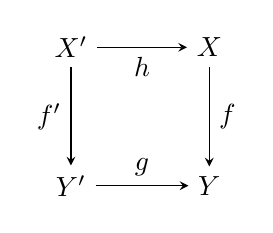
\begin{tikzpicture}[node distance=5em, auto]
					\node (A) 									{$X'$};
					\node (B) 	[right of=A]		{$X$};
				  \node (C) 	[below of=A]	 	{$Y'$};
				  \node (D) 	[below of=B] 		{$Y$};
				  \draw[-stealth][swap]		(A)		to node {$h$} 				(B);
				  \draw[-stealth]					(C)		to node {$g$} 				(D);
				  \draw[-stealth][swap]		(A)		to node {$f'$} 				(C);
				  \draw[-stealth]					(B)		to node {$f$} 				(D);
				\end{tikzpicture}
			$}
		\end{tabular}
		Then for every base change diagram as above, setting $\scr{F}'=h^*\scr{F}$, the natural map $g^* R^i f_* \scr{F} \to R^i f'_*\scr{F}'$ is an isomorphism for every $i\geq 0$.
	\end{prop}
	\begin{proof}
		First observe that on fibres, for every $y\in Y$ and $y'\in Y'$ such that $g(y')=y$, we have isomorphisms
		\begin{equation}\label{eq:fibres}
			H^i(X_y, \scr{F}_{\mid y}) \cong H^i(X_{y'}, \scr{F'}_{\mid y'}) \qquad \forall\; i\geq 0\;.
		\end{equation}
		Next, applying Proposition \ref{prop:no_jumps} and using induction from above, we readily see that our hypothesis of the vanishing of $R^if_*\scr{F}$ in positive degrees implies that
		$$ 
		H^i(X_y, \scr{F}_{\mid y}) = 0 \quad \forall\;i>0 
		\AND 
		H^0(X_y, \scr{F}_{\mid y}) \cong f_* \scr{F}_{\mid y} \;.
		$$ 
		Further, combining the above with \eqref{eq:fibres}, we deduce that the function $y'\mapsto h^i(X_{y'}, \scr{F'}_{\mid y'})$ is constantly equal to zero $\forall\; i>0$, hence -- invoking Proposition \ref{prop:no_jumps} again -- it follows that $R^i f_*' \scr{F}'$ vanishes for positive $i$ and, moreover, that
		$$ H^0(X_{y'}, \scr{F'}_{\mid y'}) \cong f_*'\scr{F}'_{\mid y'} \qquad \forall\; y' \in Y'. $$
		Therefore we deduce -- we can apply Proposition \ref{prop:no_jumps} since $f_*\scr{F}$ is locally free -- that the function
		$$ y'\mapsto h^0(X_{y'}, \scr{F'}_{\mid y'}) = h^0(X_y, \scr{F}_{\mid y}) $$
		is also constant, hence $f_*'\scr{F}'$ is locally free. Since pullbacks preserve locally free sheaves, the sheaf $g^* f_*\scr{F}$ is locally free as well and, as a consequence, we have
		$$ g^* f_* \scr{F}_{\mid y'} = f_* \scr{F}_{\mid y} \cong H^0(X_y, \scr{F}_{\mid y}). $$ 
		Now, for $i>0$ we are done, while for $i=0$ we have a natural map $g^* f_* \scr{F} \to f'_*\scr{F}'$ between two locally-free sheaves. Form the above discussion combined with \eqref{eq:fibres}, it follows that the two sheaves are fiberwise isomorphic and, further, one can check that the isomorphisms on fibres are induced by the natural map, thus getting to the desired conclusion.
	\end{proof}
	\vspace{1em}
	%
	We continue this Section by proving an easy Lemma, which is used more than once during our discussion. The idea is that to kill the higher cohomology of a family of line bundles it is enough to add a divisor of high degree, then the \RR finishes the job.
	\begin{lemm}\label{lemm:trivial_R1}
		Let $X$ be a smooth projective curve over an algebraically closed field, let $T$ be an $S$-scheme and $L$ a family of line bundles of degree $d$ parametrised by $T$. Denote by $\phi:X_T\to T$ the natural projection, pick a divisor $D\subset X$ of degree higher than $2g-d-1$ and let $\Gamma := \phi^* D$ be the product divisor on $X_T$. Then
		$$ R^i\phi_* L = 0 \qquad \forall \;i \geq 1 $$
	\end{lemm}
	\begin{proof}
		Since over any closed point $t \in T$ the line bundle $L_{\mid t}$ has degree $d$, it follows that $L(\Gamma)_{\mid t}$ has degree strictly higher than $2g-2$. Hence from the \RR Theorem we deduce that the function
		$$ t \mapsto \dim H^1(X, L_{\mid t}) $$
		is everywhere vanishing and therefore Proposition \ref{prop:no_jumps} implies that $R^1\phi_* L$ is the trivial sheaf, being locally free with trivial fibres. For $i>1$ a similar argument applies: the only difference is that, since we are working on a curve, we do not even need to invoke the \RRo.
	\end{proof}

	Another well known and useful result is the so called Projection Formula.
	\begin{namedtheo}[Projection Formula]\label{thm:projection_formula}
		Let $f:X\to Y$ be a morphism of locally ringed spaces, $\scr{F}$ an $\OX$-module and $\cal{E}$ a locally free $\OY$-module of finite rank. Then $\forall\, i \geq 0$ we have natural isomorphisms
		\begin{equation}\label{eq:proj_formula}
			R^i f_*( \scr{F}\otimes f^* \scr{E} ) \;\cong\; R^i f_*( \scr{F}) \otimes \scr{E}
		\end{equation}
	\end{namedtheo}
	\begin{proof}
		A proof can be found in \cite[\href{http://stacks.math.columbia.edu/tag/01E8}{Lemma 01E8}]{stacks-project}. Nevertheless, we give here an alternative and more \emph{down-to-earth} proof of the result. \\
		First of all we will show that there is a natural morphism
		$$  f_*\scr{F}\otimes \scr{E} \to f_*(\scr{F}\otimes f^* \scr{E}) $$
		and, to do so, it is useful to recall the following basic results, where we denote by $\HH$ the Hom sheaf prescribed on open sets $U$ as $U\mapsto \Ho(\square_{\mid U}, \square_{\mid U})$
		\begin{enumerate}[(1)]
			\item Adjunction between $\otimes$ and $\HH$
			$$ \Ho_X(\scr{A}\otimes \scr{B},\; \scr{C}) \cong \Ho_X(\scr{A},\; \HH_X(\scr{B},\scr{C})) $$

			\item Adjunction between $f_*$ and $f^*$
			$$\Ho_Y(f_* \scr{F},\; \scr{E} ) \cong \Ho_X (\scr{F},\; f^*\scr{E})$$

			\item Identity which follows from the definitions of $\HH$ and $f_*$
		\end{enumerate}
		$$f_* \mathscr{H}_X(\scr{A},\;\scr{B}) \cong \mathscr{H}_Y(f_* \scr{A},\; f_* \scr{B})$$
		Then, the existence of the above mentioned natural map follows from the chain of isomorphisms: just pick the identity!
		\begin{eqnarray*}
			\Ho_Y(f_*\scr{F}\otimes \scr{E},\; f_*(\scr{F}\otimes f^* \scr{E})) &\overset{(1)}\cong& 
			\Ho_Y(\scr{E},\; \HH_Y(f_*\scr{F},\;f_*(\scr{F}\otimes f^* \scr{E}))) \\
			&\overset{(3)}\cong&
			\Ho_Y(\scr{E},\; f_*\HH_X(\scr{F},\;(\scr{F}\otimes f^* \scr{E}))) \\
			&\overset{(2)}\cong&
			\Ho_X(f^*\scr{E},\; \HH_X(\scr{F},\;(\scr{F}\otimes f^* \scr{E}))) \\
			&\overset{(1)}\cong&
			\Ho_X(\scr{F} \otimes f^*\scr{E},\; \scr{F}\otimes f^* \scr{E})
		\end{eqnarray*}
		We are now going to show that the obtained natural map is in fact an isomorphism. Since all the functors involved commute with open restrictions, we can reduce to the affine case and assume $\scr{E}$ is free. One can check that the above global map agrees with the chain of isomorphisms
		\begin{eqnarray*}
			f_*(\scr{F}\otimes f^*\scr{E}) 
			&\;\cong\;& f_*(\scr{F}\otimes \scr{O}_X^{\,n}) \\
			&\;\cong\;& f_*(\scr{F}\otimes \scr{O}_X)^{n} \\ 
			&\;\cong\;& f_*(\scr{F})^{n} \\
			&\;\cong\;& f_*(\scr{F})\otimes \scr{O}_Y^{\,n} \\
			&\;\cong\;& f_*(\scr{F})\otimes \scr{E}
		\end{eqnarray*}
		where we used multiple times the fact that the functors involved are additive and thus commute with finite direct sums. The obtained isomorphism implies that
			$$ R^i f_*(\scr{F}\otimes f^*\scr{E}) \;\cong\; R^i (f_*(\scr{F})\otimes \scr{E}) \;\cong\; R^i f_* (\scr{F}) \otimes \scr{E} $$
			 for every $i\in \N$. For the second isomorphism we used the well known fact that \emph{tensoring with a locally free module} is an exact functor.
	\end{proof}

\section{Line Bundles}
	In Section \ref{sec:ampleness} we need to show that a certain line bundle of interest is ample and, to do so, we exploit the combination of the following criterions for ampleness together with the next Lemma.
	\begin{prop}\label{prop:Nakai}
		Let $f:X\to Y$ be a finite and surjective morphism between proper Noetherian schemes and $L$ a line bundle over $Y$. Then $L$ is ample \ABiff its pullback $f^*L$ is.
	\end{prop}
	\begin{proof}
		We refer to \cite{HAG}, where the result is given in Ex. III.5.7.d.
	\end{proof}

	\begin{prop}\label{prop:Nakai_Moishezon}
		Let $Y$ be a smooth projective surface. Then the line bundle corresponding to a Cartier divisor $D$ is ample \ABiff the self-intersection number $D^2$ is strictly positive and $C\cdot D >0$ for every irreducible curve $C\subset Y$. 
	\end{prop}
	\begin{proof}
		We refer to \cite{HAG}, Theorem V.1.10.
	\end{proof}


	\begin{lemm}\label{lemm:tensor_ampleness}
		For every $i=1,\dots n$, let $Y_i$ be a smooth projective curve over an algebraically closed field $k$ and $M_i$ an ample line bundle on $Y_i$. Further let $Y=Y_1\times\dots\times Y_n$ and denote by $\pi_i:Y \to Y_i$ the projection on the $i$-th component. Then the line bundle
		$ \otimes_{i=1}^n \pi_i^* M_i $
		over $Y$ is ample.
	\end{lemm}
	\begin{proof}
		We will prove the claim for the case $n=2$, then the general result easily follows by induction over $n$. Notice that $Y_1 \times Y_2$ is a smooth projective surface. \\

		Set $L=\pi_1^*M_1 \otimes \pi_2^*M_2$. Since $M_1$ and $M_2$ are ample, replacing $L$ with $L^{\otimes m}$ with $m$ big enough ( if needed ) we see that $L$ admits a section which corresponds to the effective divisor
		$$ D = \sum_a F_a + \sum_b G_b $$
		where each $F_a$ is a fiber of $\pi_1$ and each $G_b$ is a fiber of $\pi_2$. Notice that, since the surface $Y_1 \times Y_2$ is the product of two curves, all such fibres are algebraically equivalent. Hence, given an irreducible curve $C\subset Y$, we can choose the fibres $F_a$ and $F_b$ in such a way that the intersection between $C$ and $D$ is proper, so that we get $C\cdot D > 0$. Moreover, this argument applies to the case $C=D$ as well, therefore also $D^2>0$ and by Proposition \ref{prop:Nakai_Moishezon} we conclude that $L$ is ample.
	\end{proof}	


	\begin{comment}
		\begin{lemm}\label{lemm:tensor_ampleness}
			Let $X$ be a proper Noetherian variety and $L_1, \dots, L_m$ a finite number of ample line bundles over $X$. Then their tensor product $ \otimes_{i=1}^m L_i $ is ample.
		\end{lemm}
		\begin{proof}
			We will prove the claim for a pair of line bundles $L$ and $M$, then the general result easily follows by induction over $m$.\\

			Since $X$ is proper and Noetherian the Cartan-Serre-Grothendieck Theorem holds and, thus, an equivalent condition for the ampleness of $L$ is the existence of a natural number $m\in \N$ such that for every coherent sheaf $\scr{F}$ on $X$ we have
			$$ H^i(X, \scr{F}\otimes L^{\otimes n}) = 0 \qquad \forall \; i\geq 1 \,. $$
		 	Now let $\scr{E}$ be any coherent sheaf on $X$ and notice that, in particular, the above condition holds for the coherent $\scr{F} = \scr{E}\otimes M^{\otimes n}$. Therefore for every $i\geq 1$ we find
		 	$$ H^i(X, \scr{E}\otimes (L\otimes M)^{\otimes n} ) = H^i(X, \scr{F}\otimes L^{\otimes n} ) = 0 $$
		 	and, hence, by another application of the Cartan-Serre-Grothendieck Theorem we see that $L\otimes M$ is ample.
		\end{proof}	
	\end{comment}	

	We now prove a Lemma about the behaviour of line bundles over a product with a complete factor, which we use in Section \ref{sec:defi_modu}.
	\begin{lemm}\label{lemm:square}
		Let $X$ and $Y$ be schemes, with $X$ complete and $L,M$ line bundles over $X\times Y$ such that $\forall y\in Y$ we have $L_y \cong M_y$. Then there exists a line bundle $F$ over $Y$ such that $L\cong M\otimes \pi^* F$, where $\pi :X \times Y\to Y$ is the natural projection.
	\end{lemm}
	\begin{proof}
		Let $F=L\otimes M^{-1}$ and notice that, since $F_y$ is trivial and $X$ is complete, for every $y\in Y$ we have $H^0(X, F_y)=k(y)$. Hence the function
		$$ y \mapsto \dim_{k(y)} H^0(X, F_y) $$
		is constantly equal to $1$. Therefore, by Proposition \ref{prop:no_jumps}, $\pi_* F$ is locally free of rank $1$, i.e.\ it is a line bundle over $Y$. Now, if we show that the natural map 
		$$ \ph: \pi^*\pi_* F \to F $$
		is an isomorphism, we are done. On every fiber the above map restricts to the isomorphism
		$$ \OX \otimes H^0(X, \OX) \toiso \OX $$
		so by Nakayama's lemma we deduce that $\ph$ is surjective. But rank is invariant under pullback, so $\pi^* \pi_* F$ has rank $1$, thus forcing $\ph$ to be an isomorphism.
	\end{proof}

	Finally, we prove that line bundles on $X_T/T$ with the canonical rigidification discussed in Section \ref{sec:Pic_functor} admit no nontrivial automorphisms. This is the main reason why one defines the relative Picard functor as in Section \ref{sec:Pic_functor}, since the absence of automorphisms allows for its representability.
	\begin{prop}\label{prop:rigid}
		Under hypothesis and notation of $(\star)$ from Section \ref{sec:assumptions}, line bundles on $X_T/T$ with the canonical rigidification along $\eps_T$ have no nontrivial automorphisms. 
	\end{prop}
	\begin{proof}
		First of all, to make the setting clear, let us draw the fibered diagram we are working with, filled with the sections we have at our disposal (we  abuse notation and write $\eps$ also for the pullback morphism $\eps_T$). Further, we draw the diagram describing a morphism of line bundles with rigidification on the right.
		
		\begin{equation*}
		\begin{tikzpicture}[node distance=5em, auto] %SQUARE
			\node (A) 															{$X_T$};
			\node (B) 	[right of=A, xshift=3em]		{$T$};
		  \node (C) 	[below of=A] 								{$X$};
		  \node (D) 	[right of=C, xshift=3em] 		{$S$};
		  %
		 	\node (A2) 	[right of=B, xshift=3em]			{$\calO_T$};
			\node (B2) 	[right of=A2, xshift=2em]			{$\eps^*L_1$};
		  \node (C2) 	[below of=A2] 								{$\calO_T$};
		  \node (D2) 	[right of=C2, xshift=2em] 		{$\eps^*L_2$};
		  %
		  \draw[-stealth, bend left=15, looseness=1]						(A)		to node {$f$} 			(B);
		  \draw[-stealth, bend left=15, looseness=1]						(B)		to node {$\eps$} 	(A);
		  \draw[-stealth]																				(A)		to node {} (C);
		  \draw[-stealth]																				(B)		to node {} (D);
		  \draw[-stealth, bend right=15, looseness=1, swap]			(D)		to node {$\eps$}		(C);
		  \draw[-stealth, bend right=15, looseness=1, swap]			(C)		to node {$f$} 			(D);
		  %
		  \draw[-stealth]						(A2)		to node {$\al_1$} 				(B2);
		  \draw[-stealth, swap]			(A2)		to node {$=$} 						(C2);
		  \draw[-stealth]						(B2)		to node {$\eps^*\ph$} 	(D2);
		  \draw[-stealth, swap]			(C2)		to node {$\al_2$}					(D2);
		\end{tikzpicture}
		\end{equation*}
		
		Recall that a morphism between two line bundle with rigidification $\ph:(L_1,\al_1) \to (L_2,\al_2)$ consists of a morphism of (plain) line bundles $\ph:L_1\to L_2$ such that $(\eps^* \,\ph)\,\al_1 = \al_2$ and, in particular, an endomorphism is an element $h\in \Gamma(X_T, \calO_{X_T})$ such that $\eps^* \,h = 1$. But from of our assumption $f_*\calO_{X_T} \cong \calO_T$, contained in $(\star)$, we get isomorphisms
		$$ \Gamma(X_T, \calO_{X_T}) \cong \Gamma(T, f_*\calO_{X_T}) \underset{(\star)}\cong \Gamma(T, \calO_{T}) $$
		and we therefore see that the only automorphisms are the trivial ones.
	\end{proof}

\section{Tangent space of schemes}
	The following basic lemmata allow us to compute the tangent spaces of the schemes $\EDiv_X$ and $\Pic_X$ in Section \ref{sec:tgnt_spaces}. Recall that we use the notation $k_\eps$ for the ring of dual numbers $k[\eps]/\eps^2$.
		\begin{lemm}\label{lemm:tng_sch}
		Let $P$ be a scheme over $S=\Spec(k)$ locally of finite type and $e\in P$ a rational point. Then we have an isomorphism of vector spaces
		$$ P(k_\eps)_e \; \cong \; T_e P. $$
	\end{lemm}
	\begin{proof}
		Let $\frakm$ be the maximal ideal of $e$ and $A$ its local ring. The Zariski tangent space at $e$ is $\Hom(\frakm/\frakm^2, k)$, which can naturally be identified with the set of $k$-derivations $\delta:A\to k$. To any such derivation corresponds bijectively a $k$-map
		$$ u_\delta : A \to k_\eps, \quad a\mapsto a \text{ mod } \frakm + \eps\delta(a), $$
		as it is easy to show. Further, any such map gives rise to a unique map of schemes
		$$ t_\delta : \Spec(k_\eps) \to P $$
		which is supported at $e$, and viceversa. Therefore we proved that $P(k_\eps)_e \cong T_e P$ as sets. We now want to see how the vector space structure of $T_e P$ transfers to $P(k_\eps)_e$, starting from the multiplication by scalars. For $b\in k$ it is easy to check that the $k$-map
		$$ \mu_b : k_\eps\to k_\eps, \quad \eps \mapsto b\cdot \eps $$
		corresponds to multiplication by $b$ in $T_eP$. Therefore scalar multiplication by $b$ on $P(k_\eps)_e$ is given by the map
		$$ P(\mu_b) : P(k_\eps)_e \to P(k_\eps)_e. $$
		For the additive structure, first define $k_{\eps,\eps'}$ to be the ring obtained by adjoining to $k_\eps$ an element $\eps'$ such that $\eps'^2 = \eps\eps' = 0$. Secondly define maps $\sigma_1,\sigma_2 : k_{\eps,\eps'}\to k_\eps$ by
		$$ \sigma_1: \eps\mapsto \eps,\; \eps'\mapsto 0, \qquad \sigma_2: \eps\mapsto 0,\; \eps'\mapsto \eps $$
		and use them to get a bijection $\pi:P(k_{\eps, \eps'})_e \toiso P(k_\eps)_e \times P(k_\eps)_e $. Further, let
		$$ \sigma: k_{\eps,\eps'}\to k_\eps, \qquad \eps\mapsto \eps,\; \eps'\mapsto \eps $$
		and finally set $\al = P(\sigma)\circ \pi^{-1}$. It is now a triviality to check that $\al$ corresponds to summation in $T_eP$.
	\end{proof}
	\begin{comment}
		It would be nice to give here a geometrical interpretation of the above result, together with a picture.
	\end{comment}
	In the case of a group scheme we can state a slightly more powerful result:
	\begin{lemm}\label{lemm:tng_grp_sch}
		Let $P$ be a group scheme over $S=\Spec(k)$ locally of finite type and $e\in P$ the identity element. Then we have an isomorphism of vector spaces
		$$ T_e P \;\cong\; \ker \Big( P(k_\eps) \to P(k) \Big). $$
	\end{lemm}
	\begin{proof}
		The natural map of rings $k_\eps \to k$ gives rise to a map of schemes $\rho: P(k_\eps) \to P(k)$ whose kernel is $P(k_\eps)_e \cong T_e P$. So to conclude we just need to show that the sum on $T_eP$ corresponds to the group operation of $\ker(\rho)$, i.e., using the notation of the previous lemma, that we have
		$$ \al(m,n)= m \cdot n. $$
		Let $i:k_\eps \to k_{\eps,\eps'}$ be the natural inclusion and notice that the map $\sigma_2 \circ i$ factors via $k_\eps\to k$. Thus for every $m\in P(k_\eps)_e$ we find $P(\sigma_2)\circ P(i)(m)=e$. Moreover the maps $\sigma\circ i$ and $\sigma_1\circ i$ coincide with the identity of $k_\eps$, which implies
		$$ P(\sigma)\circ P(i)(m)=m \AND \pi\circ P(i)(m) = (m,e). $$
		Hence we deduce
		$$ \al(m,e) = P(\sigma)\circ \pi^{-1}(m,e) = P(\sigma)\circ P(i)(m) = m $$
		and similarly $\al(e,n) = n$. Since $\al$ arises from the composition of two ring homomorphisms, it is a group homomorphism and therefore
		$$ \al(m,n) = \al(m,e)\cdot\al(e,n) = m\cdot n $$
		as desired.
	\end{proof}

\section{Clifford's Theorem}

	This Section is dedicated to the famous Theorem of Clifford, which gives an upper bound on the dimension of linear series. In order to prove it, we first need some preliminary results.
		\begin{lemm}
		For a divisor $D$ on a curve $X$ we have $\dim|D|\geq k$ \ABiff for every set of $k$ points $p_1, \dots, p_k$ of $X$ there exists an element of $|D|$ containing all of them.
	\end{lemm}
	\begin{proof}
		If for every set of $k$ points $p_1, \dots, p_k$ of $X$ there exists a divisor in $|D|$ containing all of them, then trivially $\dim|D|\geq k$ since the family $\sum_{i=1}^d p_i$ is $k$-dimensional.\\
		Conversely, assume $\dim|D|\geq k$ and pick $k$ points $p_1, \dots, p_k$ of $X$. We have 
		$$ h^0(X, D - \sum_{i=1}^d p_i) \geq h^0(X, D) - k \geq 1, $$
		so that there exists a global section $f\in H^0(X, D - \sum_{i=1}^d p_i)$ such that 
		$$ (f)+D-\sum_{i=1}^d p_i \geq 0 \iff D' = (f)+D \geq \sum_{i=1}^d p_i, $$
		therefore $D'$ is an element of $|D|$ containing all the points.
	\end{proof}
	\begin{coro}
		Let $D_1$ and $D_2$ be two effective divisors of $X$. Then
		$$ \dim|D_1| + \dim|D_2| \leq |D_1+D_2|. $$
	\end{coro}
	\begin{proof}
		Assume $d_i=\dim(D_i)$ and let $p_1,\dots,p_{d_1}$ and $q_1,\dots,q_{d_2}$ be points of $X$. Then by the lemma we can find divisors $D_1'\in |D_1|$ and $D_2'\in |D_2|$ containing respectively $p_1,\dots,p_{d_1}$ and $q_1,\dots,q_{d_2}$. Therefore the divisor $D_1'+D_2' \in |D_1+D_2|$ contains all of the $d_1+d_2$ points and, applying the lemma again, we find
		$$ \dim|D_1 + D_2| \geq d_1 + d_1. $$
	\end{proof}
	We now state another useful Lemma, for which we need the following well-known fact about the non-degeneracy of the canonical image
	\begin{prop}
		Let $d\leq g$, and $X$ a curve of genus $g$. Then any $d$ points of the canonical image $\phi(X)$ are linearly independent, i.e. they span a $\PP^{d-1}.$
	\end{prop}
	\begin{lemm}\label{lemm:hyp_linear}
		Let $X$ be a hyperelliptic curve of genus $g$, and $d\leq g$. Then any complete $g_d^r$ on $X$ is of the form
		$$ r\cdot g_2^1 + P_1 + \dots + P_{d-2r}, $$
		where none of the $P_i$ is conjugate under the hyperelliptic involution.
	\end{lemm}
	\begin{proof}
		Almost immediate using the above proposition.
	\end{proof}
	Now we are almost ready to prove the crucial Clifford's theorem, which gives a bound to the dimension of the complete linear system $|D|$. But first we need another classical result, i.e.\ the
	\begin{namedtheo}[General Position Theorem]\label{thm:GPT}
		Let $r\geq 2$ and $X\subset \PP^r$ be an irreducible nondegenerate curve of degree $d$. Then a general hyperplane cuts $X$ in $d$	points, any $r$ of which are linearly independent.
	\end{namedtheo}
	A proof of the above theorem can be found in \cite{GAC}. Next, we finally move to the
	\begin{namedtheo}[Clifford's Theorem]\label{thm:Clifford}
		Let $D$ be an effective divisor on a curve $X$ with $d = \deg(D) \leq 2g-2$. Then we have:
		\begin{enumerate}[(i)]
			\item $ \dim|D| \leq \frac{d}{2}. $
			\item The equality holds only if $D=0$, $D=K$ or, in case $X$ is hyperelliptic, if $D$ is a multiple of the hyperelliptic involution.
		\end{enumerate}
	\end{namedtheo}
	\begin{proof}
		Before beginning with the proof, recall that a divisor $D$ is called \textbf{special} if $h^0(K-D) > 0$.
		\begin{enumerate}[(i)]
			\item If $D$ is not special then by the \RR we get
			$$ h^0(D) = d-g+1 \iff \dim|D| = d-g $$
			which by hypothesis is strictly lower than $d/2$, since $g \geq d/2+1 $. If $D$ is special, instead, there exists an effective divisor $D'$ such that $K=D+D'$. Therefore applying the above corollary we find
			$$ \dim|D| + \dim|D'| \leq \dim|K| = g-1.  $$
			Moreover, since $D' = K-D$, the Riemann-Roch formula gives
			$$ \dim|D| - \dim|D'| = d - g + 1. $$
			Adding up the two equations we obtain the result.
			
			\item If the equality holds we have
			$$ r(D) + r(D') = g-1.  $$
			Since the degree of $K=D+D'$ is $2g-2$, without losing generality we can assume $\deg(D)\leq g-1$ and from part (i) it follows that 
			$$ r(D)=0 \implica \deg(D')=2g-2 \implica D\sim 0. $$ 
			Otherwise, let $r(D)>0$ and suppose $X$ is not hyperelliptic. From the geometric \RR we know that any hyperplane of $\PG$ cuts $X$ in $\deg(D)\leq g-1$ points of $E\in|D|$ which are not independent (recall that $r(D)>0$ means there is at least one linear relation among them). But this contradicts the general position theorem, therefore $r(D)>0$ forces $X$ to be hyperelliptic. In this case using Lemma $\ref{lemm:hyp_linear}$ we know that any complete $g_d^r$ on $X$ is of the form
			$$ |D| = r\cdot g_2^1 + P_1 + \dots + P_{d-2r} $$
			and, since we are assuming $d=2r$, we see that $|D|$ is a multiple of the hyperelliptic involution.
		\end{enumerate}
	\end{proof}

